\chapter{}
I awakened Tuesday morning, and thought I was still dreaming. Lying next to me, still
asleep, was a beautiful woman. She was encased in bright pink fiberglass from her neck to her
waist, including both arms. She wasn't injured. She was wearing the casts for her enjoyment. And
mine.

I watched her sleep for a few minutes, just taking in her beautiful face, the soft sounds
of her breathing, and the fabulous cast. I noticed how her fingers relaxed in a slightly curled
position. I noticed the smooth but distinct swell where the cast covered her chest, the small
gap at the front of the opening for her neck. It wasn't much of a gap; perhaps enough to slip a
finger in to the second knuckle. Despite my enjoyment of the situation, I was bothered by one
thing: I was living a lie to Monique. She didn't know that the rich benefactor behind my work
was actually me. I had to tell her, even if it meant hurting her and possibly losing her. I was
beginning to care about her too much to deceive her any longer. She had to know the truth, and I
hoped she could understand and forgive my deception.

She woke up and looked over at me. She smiled, and I couldn't help but smile back. I
realized that this wasn't lust, and this wasn't a good friendship. Well, actually, it WAS lust,
and it WAS a good friendship, but it was more. I was falling for her. I wasn't having the silly
teenage feelings I'd felt before. This was more comfortable, more natural. It just felt good,
and felt like it was supposed to be.

``Good morning,'' she said.

``Good morning, yourself,'' I answered. ``How did you sleep?''

``Like a rock. I don't think I moved at all,'' she replied, with a smile and a twinkle in her
eye.

``Ha ha,'' I said dryly. ``Are you ready to get out of that and go hit the park?''

``Yes, but I want another one of these sometime. I'd like a little more time in a cast like
this.''

``I promise, you can have another one any time you like,'' I told her.

``Alright, but I want the next one to be plaster.''

I got out of bed and checked the time. It was already past ten, so we figured that most of
the hotel's guests would be out of the hotel and in the park by now. We decided to get her out
of the big cast, and head out into the park before housekeeping showed up.

In the bathroom, I cut the cast perfectly in half, though I knew we couldn't save it. When
she was out of the cast, I left her to shower, and set about folding up the pieces of the cast
until they fit into a trash bag. After she was ready, I showered, and we headed downstairs to
breakfast.

\begin{thought}
As Quinn was showering, Monique looked at the lumpy trash bag that held the remains of her
double shoulder spica cast. She really had wanted more time in the cast. It was so restrictive,
and she found the helplessness exquisite. She was totally at Quinn's mercy, depending on him for
just about everything, casted like that. She was definitely going to hold him to his promise of
a repeat of the cast, but in plaster. The trip had been awesome so far, and would only get
better. She loved the casts she'd worn, but for drying speed they had used fiberglass, and she
really preferred plaster. Fiber was good, but plaster was definitely better.
\end{thought}

Once in the park, we got the wheelchair and passes that we'd gotten the day before. We took
in the rides, especially the coasters. Cedar Point is widely regarded as the number one park for
coaster enthusiasts, and we were both certainly in our element there. The variation in the
coasters is phenomenal, from the world's tallest coaster with its catapult launch to a 40 year
old wooden coaster that was almost a time machine. I'd been here before, and had ridden all of
the rides before, but never with Monique. Being with this fantastic woman made it all the more
enjoyable.

We stopped for lunch late in the afternoon. As we were eating, I looked over and saw the
huge sign at the entrance to Millennium Force. We both really love that coaster, and looking at
the sign gave me an idea.

``Monique, how would you like a sketch of yourself made right here in the park?''

``Did an idea just pop into your head?'' she asked.

``Yes. Would you mind waiting here, while I run back to the room for my pad and pencil?''

``Sure, just don't be too long. There are some coasters I want to ride again, including that
one,'' she said, pointing to the entrance that had inspired me.

``I'll be quick, and we can stay as long as we want, really. Sit tight, I'll be right back.''

``I'll be right here,'' she said, flashing that smile at me.

I hurried to the hotel room and got my paper and pencil. Housekeeping was in the room when
I entered, but that wasn't a problem since I'd stored the supplies and cut off casts in the
trunk of the car before we'd gone into the park.

I returned to Monique, pushed her over in front of the sign, and did a quick sketch of her
sitting there. When it was finished, I showed it to her. She nodded in approval, and we stashed
the drawing in a coin operated locker, and went to go ride the coaster. It was a little
difficult to get her casted foot into the car, due to the design, but it was well worth it- 310
feet tall, traveling 90+ miles per hour with a beautiful woman who I was beginning to care quite
a bit for. And she also loves to wear casts. Life does not get much better than this!

We stayed at the hotel through the end of the week. We spent our days in the park, and each
night before we returned to the hotel, we walked along the beach. We'd learned after the first
night to wrap her cast in a plastic bag to keep the sand out.

Each night, as we lay in bed, talking and cuddling, I found myself wanting more and more to
make love with her. Not because she was so beautiful, and not because she was wearing a rapidly
dirtying cast. I wanted her because my feelings for her were growing strong. Very strong. Strong
enough to justify what we both knew was going to happen soon.

Friday night, the sexual tension was becoming very intense. I knew I had to do one last
thing before we could take that step. I had to tell her the truth about myself. All of it. All
during our walk along the beach that evening, I was thinking about this, and she noticed that I
was distracted. She'd asked several times if something was on my mind. When we returned to our
room, I knew it was time. I sat her down, looked into her eyes, and just said it straight out.

``Monique, there is no man behind this. No rich benefactor paying me to do what I do. It's
all been me.'' I explained to her about my family and my inheritance.

In her eyes, I saw hurt, and I saw some anger.

``You lied to me,'' she said quietly.

``Yes. I did lie to you. I hope you can understand why I wasn't honest at the time. At that
point, I thought you were nothing but an employee. Honestly, at that time, my financial
situation really wasn't your business.''

``I know you're right, but it still stings,'' she said, standing up.

``I'm sure it does. I can only tell you that I'm sorry that I've hurt you. When I met you, I
had no idea what kind of person you are. I didn't even have any expectation or intention of
finding out what kind of person you are. If I had known, I'd have been honest up front. The
thought of hurting you a little hurts me a lot. I really mean that. It hurts me because I care
for you a lot. The feelings are getting stronger for me, and I couldn't go one minute more
without telling you.''

The look in her eyes was hard to read just then. I never wished more in my life, before or
since, to be able to read someone's mind. She walked over to where her shoes were. She slipped
her right foot into the sandal, and then the casted left foot into the cast shoe. As she bent
down to fasten the straps, I went on.

``This may sound trivial or whiny, but all my life, I've been treated differently because of
my family's money, and I hate it. People kiss my ass because of it- Until you, I've never known
a woman who seemed to care for me as a person, but rather cared for me as a rich person. It
disgusts me.''

``Quinn, my head is really spinning right now,'' She said. I need some air, and I need some
time to think. I'm going for a walk.'' She limped over to me, kissed me on the cheek, and walked
out the door.

After she'd left, I just sat there. I truly didn't know what was going to come next. When I
opened up to her, she closed off to me. I didn't know how seriously I had hurt her. Was this
relationship that seemed so great just an hour ago, over? I went out on the balcony, and stared
off at the lake and the lighthouse.

\begin{thought}
Out on the beach, Monique considered what she'd been told. She hated that she'd been lied
to. She hated it more that it was Quinn, who had peeled back her defenses, and inserted himself
so firmly in her heart, who had lied to her.

``But he IS right. At the time, it wasn't any of my business. At the time, I was nothing
more than a model. He doesn't act one single bit like any of the rich assholes I've known.''
\end{thought}

She walked along a while longer, talking the situation over in her head. She considered
many factors, and finally she knew what she needed to do. What she MUST do. She headed back to
the hotel.

I didn't know how long I stood on the balcony, leaning on the railing, staring and
thinking. It might have been fifteen minutes, but it felt like hours. I wondered if she would
even come back. By the standards of most people, the lie I'd told her was insignificant. But,
she was not most people. She wasn't even close. For someone as emotionally intense as Monique,
this revelation might have driven a wedge into something that I felt might last a long time.
Something that I knew she also thought might last a long time.

I was so lost in my thoughts; I didn't hear the quiet footsteps approaching me from behind.
I saw her in the corner of my eye as she walked up to the railing, and leaned against it beside
me. She stared off into the night as I had been. I turned and watched her as she spoke:

``You said you've ever known anyone who didn't feel like they cared for you because you have
money,'' she started. ``I've never known anyone who had money who cared about what I thought of
them. They always seem to think that the fact that they have money is enough of a positive
attribute to entice any woman. Every one I've known seems to think that I should worship them
because of their money.'' She turned her head to face me, and added ``until now.''

She leaned toward me, and we melted into a long passionate kiss. We parted from the kiss,
still embraced, faces close together.

``Monique, I'm falling in love with you.''

She smiled, and a tear streamed down her cheek.She made a sound that was half laugh, half
sob.

``Quinn, I'm already in love with you.''

I wiped away the tear, and the kissing began again. Our hands started exploring and
caressing each other. We went back into the room, and continued on the bed. The passion was
furious, yet even as we made love, it was not the animalistic passion you see in movies or on
television- it was the gentle, sensual act of two people who had connecting emotionally and
spiritually, now connecting physically. It was beautiful.

\begin{center}
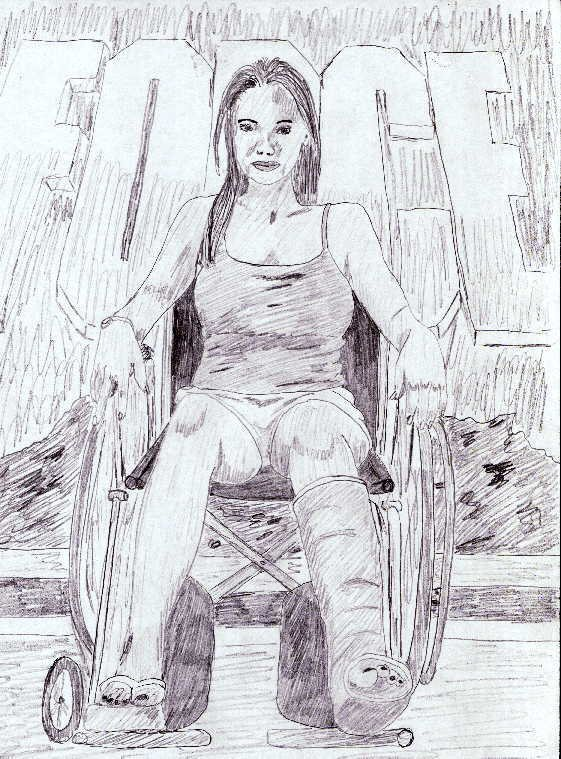
\includegraphics{images/kicks31.jpg}
\end{center}
